\section{Methods}

\subsection{Notation}

In the following, we will use definitions and notations introduced by \citet{rougier:2011} where a neural map is defined as the projection from a manifold $\Omega \subset \mathbb{R}^d$ onto a set $\mathcal{N}$ of $n$ {\em  neuron}s which is formally written as $\Phi : \Omega \rightarrow \mathcal{N}$. Each neuron $i$ is associated with a code word $\mathbf{w}_i \in \mathbb{R}^d$, all of which establish the set  $\{\mathbf{w}_i\}_{i \in   \mathcal{N}}$ that is referred as the code book. The mapping from $\Omega$ to $\mathcal{N}$ is a closest-neighbor winner-take-all rule such that any vector $\mathbf{v} \in \Omega$ is mapped to a neuron $i$ with the code $\mathbf{w}_\mathbf{v}$ being closest to the actual presented stimulus vector $\mathbf{v}$,
\begin{equation}
\Phi : \mathbf{v} \mapsto argmin_{i \in \mathcal{N}} (\lVert \mathbf{v} -
\mathbf{w}_i \rVert).
\label{eq:psi}
\end{equation}
The neuron $\mathbf{w}_\mathbf{v}$ is named the best matching unit (BMU) and the set $C_i = \{x \in \Omega | \Phi(x) = \mathbf{w}_i \}$ defines the {\em receptive field} of the neuron $i$.


%Before we present our new SOM learning algorithm, we introduce the notation  and terminology we are using throughout the present work. We borrow the notation from a previous work \citep{rougier:2011}.  A neural map is defined to be the projection from a manifold $\Omega \subset \mathbb{R}^d$ onto a set $\mathcal{N}$ of $n$ {\em neuron}s $\Phi : \Omega \rightarrow \mathcal{N}$. Each neuron $i$ is associated with a code word $\mathbf{w}_i \in \mathbb{R}^d$, all of which establish the set  $\mathcal{W} = \{\mathbf{w}_i, i \in \mathcal{N}\}$ that is referred as the code book. The mapping from $\Omega$ to $\mathcal{N}$ is a closest-neighbor winner-take-all rule such that any vector $\mathbf{v} \in \Omega$ is mapped to a neuron $i$ with the code $\mathbf{w}_\mathbf{v}$ being closest to the current input vector $\mathbf{v}$,
%\begin{equation}
%\Phi : \mathbf{v} \mapsto argmin_{i \in \mathcal{N}} (\lVert \mathbf{v} -
%\mathbf{w}_i \rVert).
%\label{eq:psi}
%\end{equation}
%The neuron $\mathbf{w}_\mathbf{v}$ is named the best matching unit (BMU) and the set $C_i = \{x \in \Omega | \Phi(x) = \mathbf{w}_i \}$ defines the {\em receptive field} of neuron $i$.


\subsection{Spatial distribution} % \& Centroidal Voronoi Tesselation}
\label{sec:spatial_dist}

The SOM space is usually defined as a two-dimensional region where nodes are arranged in a regular lattice (rectangular or hexagonal). Here, we consider instead the random placement of neurons with a specific spectral distribution (blue noise). As explained by \citet{Zhou:2012}, the spectral distribution property of noise patterns is often described in terms of the Fourier spectrum color. White noise corresponds to a flat spectrum with equal energy distributed in all frequency bands while blue noise has weak low-frequency energy, but strong high-frequency energy. In other words, blue noise has intuitively good properties with points evenly spread without visible structure (see figure~\ref{fig:sampling} for a comparison of spatial distributions).
%%
\begin{figure}[htbp]
  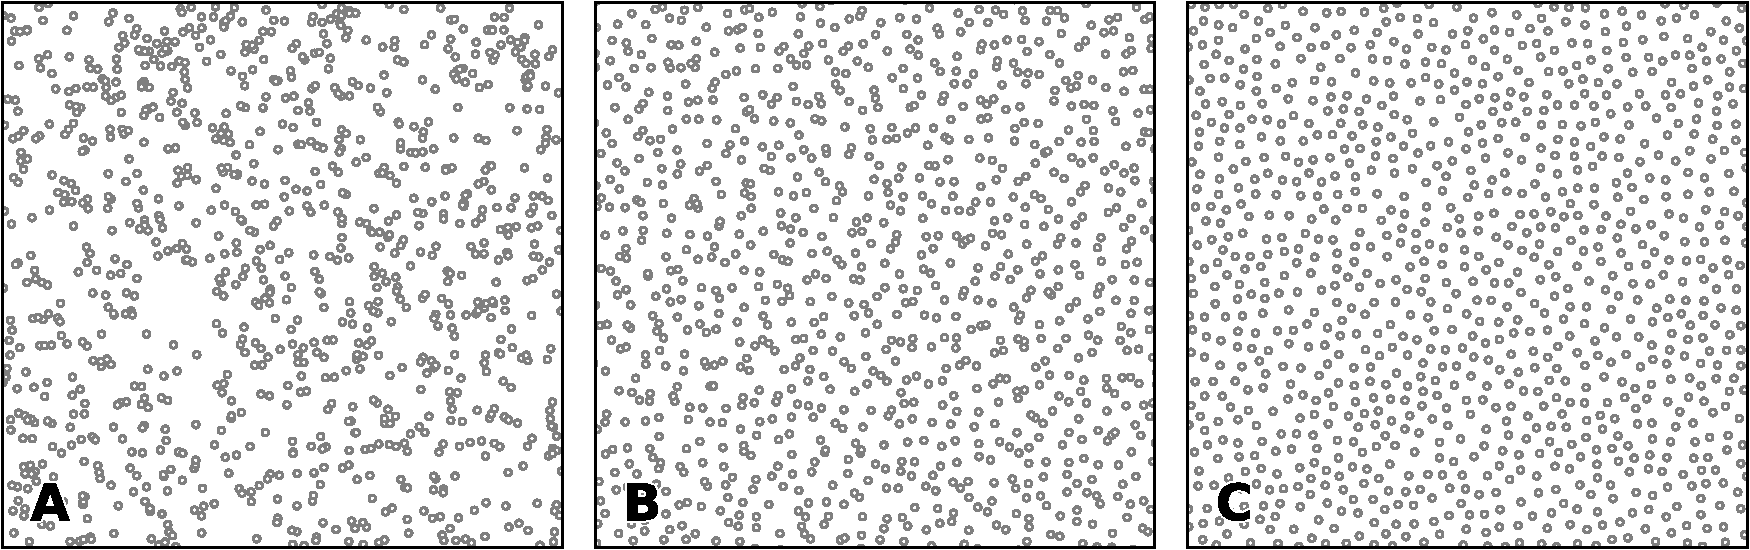
\includegraphics[width=\textwidth]{figure-blue-noise.pdf}
  \caption{\textbf{Spatial distributions.}
    \textbf{\textsf{A.}} Uniform sampling (n=1000) corresponding to white noise.
    \textbf{\textsf{B.}} Regular grid (n=32$\times$32) + jitter (2.5\%).
    \textbf{\textsf{C.}} Poisson disc sampling (n=988) corresponding to blue noise.}
  \label{fig:sampling}
\end{figure}
%%
There exists several methods \citep{Lagae:2008} to obtain blue noise sampling that have been originally designed for computer graphics (e.g. Poisson disk sampling, dart throwing, relaxation, tiling, etc.). Among these methods, the fast Poisson disk sampling in arbitrary dimensions \citep{Bridson:2007} is among the fastest ($\mathcal{O}(n)$) and easiest to use. This is the one we retained for the placement of neurons over the normalized region $[0,1]\times[0,1]$. Such Poisson disk sampling guarantees that samples are no closer to each other than a specified minimum radius. This initial placement is further refined by applying a LLoyd relaxation \citep{Lloyd:1982} scheme for 10 iterations, achieving a quasi centroidal Voronoi tesselation.


%The SOM space is usually defined as a two-dimensional manifold where nodes are arranged in a regular lattice (rectangular or hexagonal). Here, we follow a  different approach and, instead of the regular lattice, we place the neurons randomly by sampling a specific spectral distribution. More specifically, we assign neurons positions by drawing samples from a blue noise distribution. \citep{Zhou:2012}. have shown that the spectral distribution property of noise patterns is often described in terms of the Fourier spectrum color. For instance, white noise corresponds to a flat spectrum with signal's energy equally distributed to all frequency bands while blue  noise has weak low-frequency energy and strong high-frequency energy. An interesting property of the blue noise distribution is that  the resulting positions of neurons drawn are evenly spread without any apparent structure (see figure~\ref{fig:sampling} for a comparison of spatial distributions).
%%
%\begin{figure}[htbp]
%  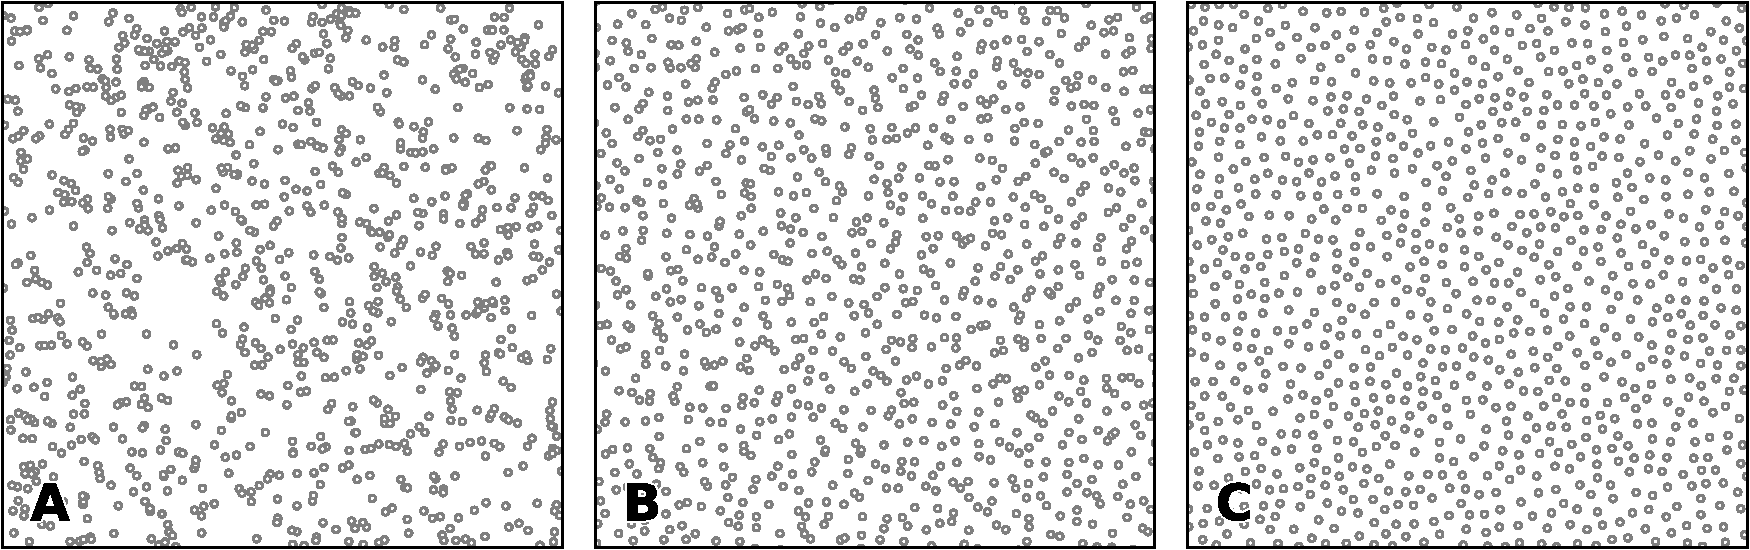
\includegraphics[width=\textwidth]{figures/blue-noise.pdf}
%  \caption{\textbf{Spatial distributions.}
%    \textbf{\textsf{A.}} Uniform sampling (n=1000) corresponding to white noise.
%    \textbf{\textsf{B.}} Regular grid (n=32$\times$32) + jitter (2.5\%).
%    \textbf{\textsf{C.}} Poisson disc sampling (n=988) corresponding to blue noise.}
%  \label{fig:sampling}
%\end{figure}
%%

%Blue noise distributions have been used in the field of computer graphics for many years and there are manych different techniques for computing them: Poisson disk sampling, dart throwing, relaxation, tiling, and other applications (see \citep{Lagae:2008} for a review). One of the fastest and easiest to implement method for generating blue noise samples is the  fast Poisson disk sampling. This method, introduced by \citet{Bridson:2007}, can be used on arbitrary dimensions in linear time ($\mathcal{O}(n)$). In this work, we propose to use this method for placing neurons over a normalized  region of $[0,1]\times[0,1]$. Such Poisson disk sampling guarantees that samples are no closer to each other than a specified minimum radius. This initial placement is further refined by applying a Lloyd relaxation~\cite{Lloyd:1982} scheme for $10$ iterations to achieve a quasi centroidal Voronoi tesselation.

\subsection{Topology}
\label{sec:topo}

Considering a set of $n$ points $P = \{P_i\}_{i \in [1,n]}$ on a finite region,
we first compute the Euclidean distance matrix $E$, where $e_{ij} = \lVert P_i - P_j \rVert$ 
and we subsequently define a connectivity matrix $G^{p}$
%= \{G^{p}_{ij}\}_{i,j \in [1,n]}$ \gid{$G^{p} = g^{p}_{ij},\, \text{where } i,j \in [1,n]$}
such that only the $p$ closest points
are connected. More precisely, if $P_j$ is among the $p$ closest neighbours of
$P_i$ then $g^p_{ij} = 1$ else we have $g^p_{ij} = 0$.
From this connectivity
matrix representing a graph, we compute the length of the shortest path between
each pair of nodes and stored them into a distance matrix $D^p$. Note that
lengths are measured in the number of nodes between two nodes such that two
nearby points (relatively to the Euclidean distance) may have a corresponding
long graph distance as illustrated in figure \ref{fig:topology}. This matrix
distance is then normalized by dividing it by the maximum distance between two
nodes such that the maximum distance in the matrix is 1. In the singular case
when two nodes cannot be connected through the graph, we recompute a spatial
distribution until all nodes can be connected.
%%
\begin{figure}
  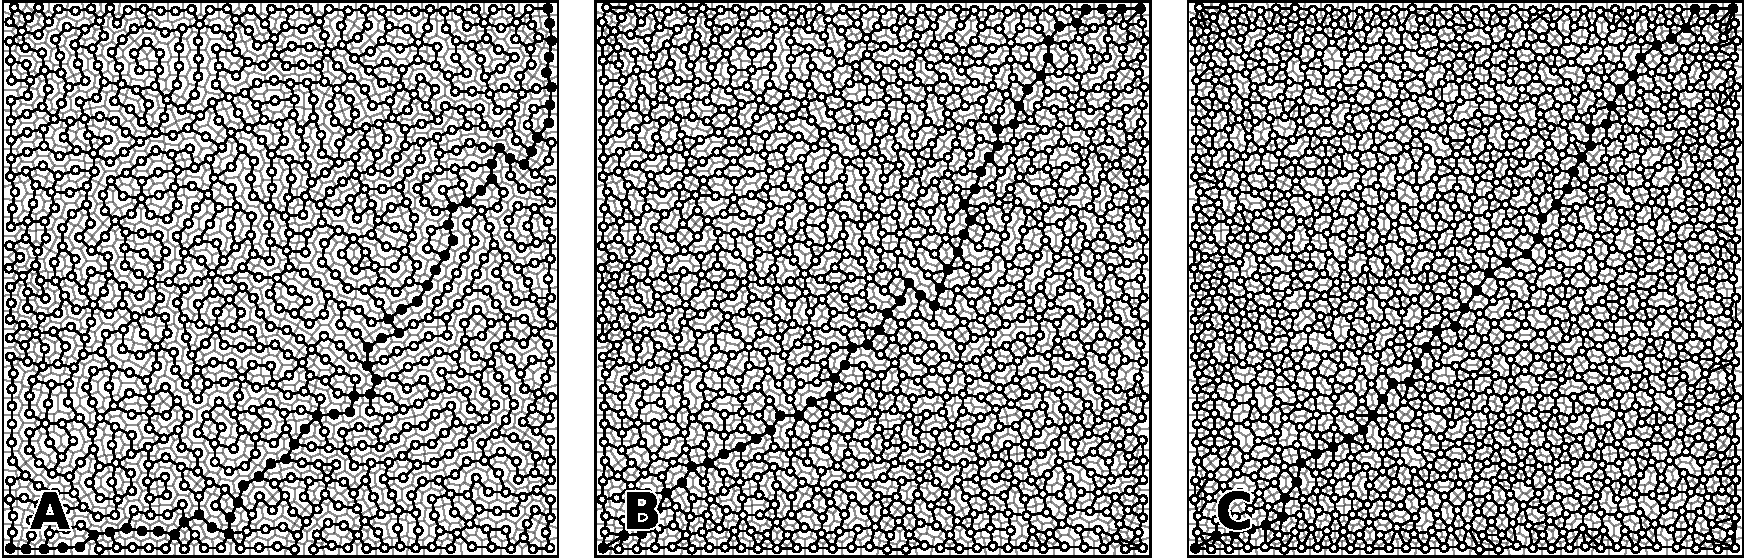
\includegraphics[width=\columnwidth]{figure-distances.pdf}
  \caption{\textbf{Influence of the number of neighbours on the graph
    distance.} The same initial set of 1003 neurons has been equiped with
    2-nearest neighbors, 3 nearest neighbors and 4-nearest neighbors induced
    topology (panels \textbf{A}, \textbf{B} and \textbf{C} respectively). A
    sample path from the the lower-left neuron to the upper-right neuron has
    been highlighted with a thick line (with respective lengths of 59, 50 and
    46 nodes).}
  \label{fig:topology}
\end{figure}

%Consider a set $P$ of $n$ points on a finite region of $[0, 1] \times [0, 1]$. The steps we follow to determine the topology of the SOM are: First, we compute the Euclidean distance matrix ${\bf E} \in \mathbb{R}^{n\times n}$, where $e_{ij} = \lVert p_i - p_j \rVert$ and $i, j=1, \ldots, n$. Subsequently  we define a connectivity matrix ${\bf G}_m$ with elements $g_{ij} = 1$ if $p_j$ belongs to the $m$ closest points to $p_i$ and $g_{ij} = 0$ otherwise. This definition implies that the matrix ${\bf G}_m$ carries information about connected neurons within a predetermined vicinity. Once we compute matrix ${\bf G_m}$, which essentially represents a graph, we compute the shortest path between each pair of nodes on the graph and we store them into a new matrix called ${\bf D}_m$. Note that lengths are measured in number of nodes (hops) required to reach two nodes such that the two corresponding Euclidean points (represented by the nodes) may have a graph distance as illustrated in figure \ref{fig:topology}.  \gid{This matrix distance is then normalized by dividing it by the maximum distance between two nodes. NOT VERY CLEAR}. In the degenerative case where two nodes are not connected on the graph, we resample from a spatial distribution until all nodes have degree greater than one (are connected at least with one other node \gid{IS THIS CORRECT?}).
%%
%\begin{figure}
%  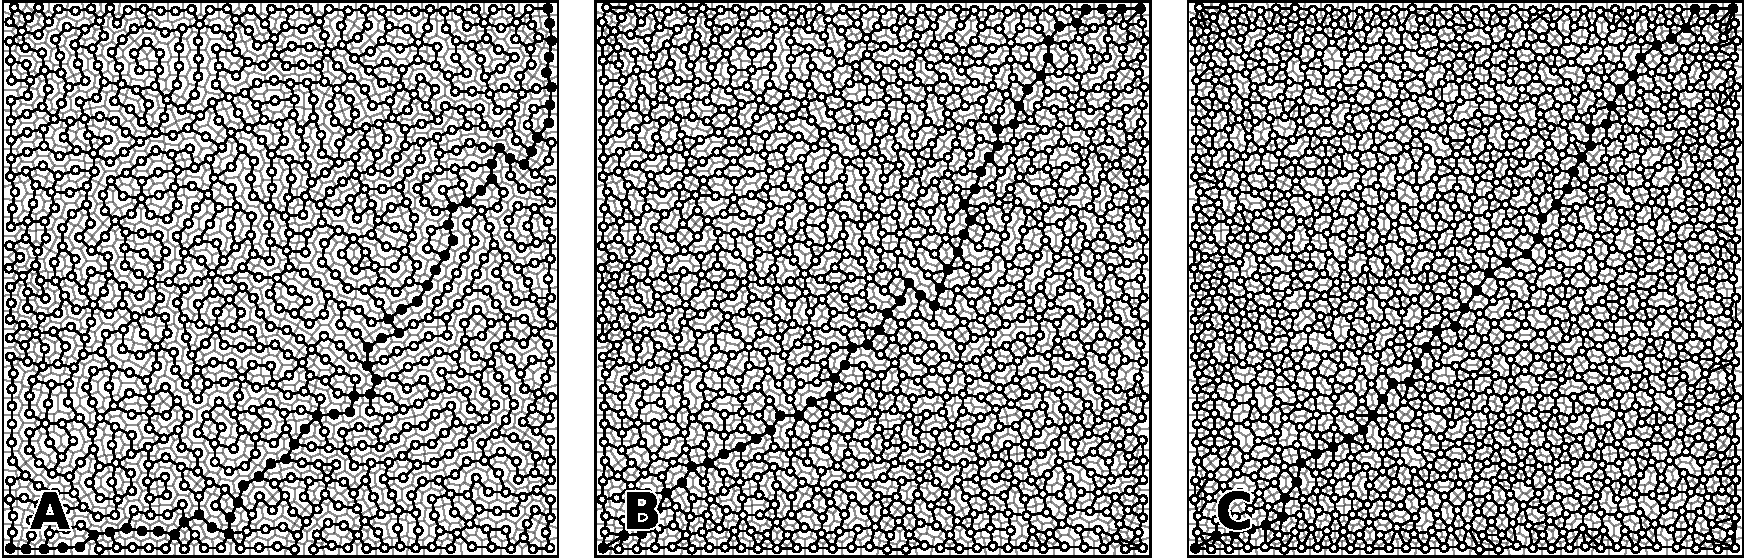
\includegraphics[width=\columnwidth]{figures/distances.pdf}
%\caption{\textbf{Influence of the number of neighbours on the graph distance.} The same initial set of 1003 neurons has been equipped with 2-nearest neighbors, 3 nearest neighbors and 4-nearest neighbors induced topology (panels \textbf{A}, \textbf{B} and \textbf{C} respectively). A sample path from the the lower-left neuron to the upper-right neuron has been highlighted with a thick line (with respective lengths of 59, 50 and 46 nodes).}
%  \label{fig:topology}
%\end{figure}


\subsection{Learning}

The learning process is an iterative process between time $t=0$ and time $t=t_f \in \mathbb{N}^+$ where vectors $\mathbf{v} \in \Omega$ are sequentially presented to the map. For each presented vector $\mathbf{v}$ at time $t$, a winner $s \in \mathcal{N}$ is determined according to equation (\ref{eq:psi}). All codes $\mathbf{w}_{i}$ from the code book are shifted towards $\mathbf{v}$ according to
\begin{equation}
  \Delta\mathbf{w}_{i} = \varepsilon(t)~h_\sigma(t,i,s)~(\mathbf{v} -
  \mathbf{w}_i)
  \label{eq:som-learning}
\end{equation}
with $h_\sigma(t,i,j)$ being a neighborhood function of the form
\begin{equation}
  h_\sigma(t,i,j) = e^{- \frac{{d^p_{ij}}^2}{\sigma(t)^2}}
  \label{eq:som-neighborhood}
\end{equation}
where $\varepsilon(t) \in \mathbb{R}$ is the learning rate and $\sigma(t) \in \mathbb{R}$
is the width of the neighborhood defined as
\begin{equation}
  \sigma(t) =
  \sigma_i\left(\frac{\sigma_f}{\sigma_i}\right)^{t/t_f}, \text{ with } \varepsilon(t) =
  \varepsilon_i\left(\frac{\varepsilon_f}{\varepsilon_i}\right)^{t/t_f},
\end{equation}
while $\sigma_i$ and $\sigma_f$ are respectively the initial and final neighborhood width and $\varepsilon_i$ and $\varepsilon_f$ are respectively the initial and final learning rate. We usually have $\sigma_f \ll \sigma_i$ and $\varepsilon_f \ll \varepsilon_i$.

%The learning algorithm we propose in this work relies on the standard SOM algorithm~\cite{Kohonen:1982}. Once we have define the topology of the map following the steps we described in paragraph~\ref{sec:topo}, we can start the learning process. Learning is iterative and starts at a time $t_0=0$ and runs until some predetermined final time step, $t_f \in \mathbb{N}^+$, has been reached. At every iteration input vectors $\mathbf{v} \in \Omega$ are sequentially given to the map with respect to the probability density function $f$ \gid{Where is defined?}. For each vector $\mathbf{v}$ at time $t$, a winner neuron with index  $s \in \mathcal{N}$ is determined according to equation (\ref{eq:psi}). This means that at time $t$ neuron $s$ is closer to the input vector ${\bf v}$, in the sense of Euclidean distance, than any other neuron. Once the winner neuron has been identified all codes $\mathbf{w}_{i}$ from the current code book are shifted towards $\mathbf{v}$ according to
%\begin{align}
%\label{eq:som-learning}
%    \Delta\mathbf{w}_{i} &= \varepsilon(t)~h(t,i,s;\sigma)~(\mathbf{v} - \mathbf{w}_i), 
%\end{align}
%where $s$ is the index of the winner neuron, $i$ is the index of code words in the code book and $t$ is the current time step. $h_\sigma(t,i,j;\sigma)$ is a neighborhood function of the form
%\begin{equation}
%  h(t,i,j; \sigma) = \exp\Big(-\frac{{d_{ij}}^2}{\sigma(t)^2}\Big)
%  \label{eq:som-neighborhood}
%\end{equation}
%where $\varepsilon: \mathbb{R} \rightarrow \mathbb{R}$ is the learning rate time-dependent function given by $\varepsilon(t) = \varepsilon_i\left(\frac{\varepsilon_f}{\varepsilon_i}\right)^{t/t_f}$, where $\varepsilon_i$ and $\varepsilon_f$ are the initial and final learning rates, respectively. $\sigma: \mathbb{R} \rightarrow \mathbb{R}$ is determines the width of the  neighborhood function~\eqref{eq:som-neighborhood} and it is reads $\sigma(t) = \sigma_i\left(\frac{\sigma_f}{\sigma_i}\right)^{t/t_f}$, where $\sigma_i$ and $\sigma_f$ are the initial and final neighborhood widths, respectively. We usually assume $\sigma_f \ll \sigma_i$ and  $\varepsilon_f \ll \varepsilon_i$. The entire learning procedure is summarized by Algorithm~\ref{algo:vsom}. 

%% %%
\begin{algorithm}[!htpb]
	\begin{algorithmic}
    	\Require $\mathcal{S}$, $\mathcal{N}$, $t_f$, $dt$, $\varepsilon_i$, $\varepsilon_f$, $\sigma_i$, $\sigma_f$
        \Ensure ${\bf W}$
        \If {\text{Blue noise is True}}
        	\State Compute blue noise distribution $\mathcal{B}$
        	\State Compute $e_{ij} = || p_i - p_j ||$		\Comment{Euclidean pair distances matrix}
        	\State Construct matrix ${\bf G}_m$			\Comment{Connectivity matrix}
        	\State Compute matrix ${\bf D}_m$			\Comment{Shortest paths between nodes}
        	\State Place neurons positions on points sampled from $\mathcal{B}$
        \Else
        	\State Discretize grid $[0, 1]\times[0, 1]$ and place neurons on its nodes
        \EndIf
        
        \State $w_s \gets \varnothing$, ${\bf W} \sim \mathcal{U}(0, 1)$	\Comment{Initialize winner unit and code book}
                 
        \For{$t \gets 0, \ldots, t_f$}
        	\State ${\bf v} \gets \bf{s}_t $	\Comment{${\bf s}_t \in \mathcal{S}$}
        	\State $s \gets argmin_{i \in \mathcal{N}} (\lVert \mathbf{v} - \mathbf{w}_i \rVert)$
        	\State $\varepsilon(t) = \varepsilon_i\left(\frac{\varepsilon_f}{\varepsilon_i}\right)^{t/t_f}$
        	\State $\sigma(t) = \sigma_i\left(\frac{\sigma_f}{\sigma_i}\right)^{t/t_f}$
        	\State $h(t,i,j; \sigma) = \exp\Big(-\frac{{d_{ij}}^2}{\sigma(t)^2}\Big)$
        	\State ${\bf w}_i^{\text{new}} = {\bf w}_i^{\text{old}} + \varepsilon(t) \odot h(t,i,s;\sigma) \odot (\mathbf{v} - \mathbf{w}_i^{\text{old}})$
        \EndFor
	\end{algorithmic}
\caption{Voronoi Self-organizing Map (vSOM). $\mathcal{N}$ is neurons index set,
$\mathcal{I}$ is the input dataset, $t_f$ is the simulation time (or the number of input samples).
$\varepsilon_i$ and $\varepsilon_f$ are the initial and final learning rates,
respectively. $\sigma_i$ and $\sigma_f$ are the initial and final neighborhood
widths. $\odot$ is the Hadamard product.}
\label{algo:vsom}
\end{algorithm}
%%


\subsection{Analysis Tools}
In order to analyze and compare the results of RSOM and SOM, we used a spectral method and persistence diagram analysis on the respective codebooks. These analysis tools are detailed below but roughly, the spectral method allows to estimate the distributions of eigenvalues in the activity of the maps while the persistence diagram allows to check for discrepancies between the topology of the input space and the topology of the map.

% To analyze the results of both the Kohonen SOM and VSOM algorithms and to make any comparison between the two algorithms we use a spectral method and persistence diagram on codebooks. The spectral method estimates the distributions of eigenvalues of the activity of neurons. The persistence diagram is a topological-geometrical  approach, more precisely is a tool coming from the field of topological data analysis (TDA). TDA provides the tools to investigate the topology of the maps and the input space and spot differences between the topology of the input space and the neural space of the SOM algorithms (Kohonen and VSOM). 

%\subsubsection{Topological Data Analysis}
\label{sec:tda}

Topological Data Analysis (TDA) \citep{Carlsson:2009} provides methods and tools to study topological structures of data sets such as point cloud and is useful when geometrical or topological information is not apparent within a data set. Furthermore, TDA tools are insensitive to dimension reduction and noise which make them well suited to analyze high-dimensional self-organized maps and their corresponding input data sets. In this work, we use the notion of persistent barcodes and diagrams \citep{Edelsbrunner:2008} to spot any differences between the topology of the input and neural spaces. Furthermore, we can apply some metrics from TDA such as the Bottleneck distance and measure how close two persistent diagrams are.
% qualify the quality of the representations of a map.
Since the exact manifold (or distribution) of the input space is not known in general and the SOM algorithms only approximate it, we simplify these manifolds by retaining their original topological structure.
Here we approach the manifolds of input and neural spaces using the Alpha complex. Before diving into more details regarding TDA, we provide here a few definitions and some notation. A $k$-simplex $\sigma$ is the convex hull of $k+1$ affinely independent points (for instance a $0$-simplex is a point, a $1$-simplex is an edge, a $2$-simplex is a triangle, etc). A simplicial complex with vertex set $\mathcal{V}$ is a set $\mathcal{S}$ of finite subsets of $\mathcal{V}$ such that the elements of $\mathcal{V}$ belong to $\mathcal{S}$ and for any $\sigma \in \mathcal{S}$ any subset $\sigma$ belongs to $\mathcal{S}$. Said differently, a simplicial complex is a space that has been  constructed out of intervals, triangles, and other higher dimensional simplices.

In our analysis we let $\mathcal{S}(\mathcal{M}, \alpha)$ be a Alpha simplicial complex with $\mathcal{M}$ being a point cloud, either the input space or the neural one, and $\alpha$ is the ``persistence'' parameter. More specifically, $\alpha$ is a threshold (or radius as we will see later) that determines if the set $X$ spans a $k$-simplex if and only if $d(x_i, x_j) \leq \alpha$ for all $0 \leq i, j \leq k$. From a practical point of view, we first define a family of thresholds $\alpha$ (or radius) and for each $\alpha$, we center a ball of radius $\alpha$ on each data point and look for possible intersections with other balls. This process is called filtration of simplicial complexes. We start from a small $\alpha$ where there are no intersecting balls (disjoint set of balls) and steadily we increase the size of $\alpha$ up to a point where a single connected blob emerges. As $\alpha$ varies from a low to a large value, holes open and close as different balls start intersecting. Every time an intersection emerges we assign a {\em birth} point $b_i$ and as the $\alpha$ increases and some new intersections of larger simplicies emerge some of the old simplicies die (since they merge with  other smaller simplicies to form larger ones). Then we assign a {\em death} point $d_i$. A pair of a birth and death points $(b_i, d_i)$ is plotted on a Cartesian two-dimensional plane and indicates when a simplicial complex was created and when it died. This two-dimensional diagram is called persistent diagram and the pairs (birth, death) that last longer reflect significant topological properties. The longevity of birth-death pairs is more clear in the persistent barcodes where the lifespan of such a pair is depicted as a straight line.

In other words, for each value of $\alpha$ we obtain new simplicial complexes and thus new topological properties such as  homology are revealed. Homology encodes the number of  points, holes, or voids in a space. For more thorough reading we refer the reader to \citep{Chazal:2017,Ghrist:2008,Zomorodian:2005}. In this work, we used the Gudhi library~\citep{Maria:2014} to compute the Alpha simplicial complexes, the filtrations and the persistent diagrams and barcodes. Therefore, we compute the persistent diagram and persistent barcode of the input space and of the maps and we calculate the Bottleneck distance between the input and SOM and RSOM maps diagrams. The bottleneck distance provides a tool to compare two persistent diagrams in a quantitative way. The Bottleneck distance between two persistent diagrams $\text{dgm}_1$ and $\text{dgm}_2$ as it is described in~\cite{Chazal:2017}
%%
\begin{align}
    \label{eq:bottle}
    d_b(\text{dgm}_1, \text{dgm}_2) &= \inf_{\text{matching }m}\{ \max_{(p, q) \in m} \{||p - q||_{\infty} \} \},
\end{align}
%%
where $p \in \text{dgm}_1 \backslash \Delta$, $q \in \text{dgm}_2 \backslash \Delta$, $\Delta$ is the diagonal of the persistent diagram (the diagonal $\Delta$ represents all the points that they die the very moment they get born, $b = d$). A matching between two  diagrams $\text{dgm}_1$ and $\text{dgm}_2$ is a subset $m \subset \text{dgm}_1 \times \text{dgm}_2$ such that every point in $\text{dgm}_1 \backslash \Delta$ and $\text{dgm}_2 \backslash \Delta$ appears exactly once in $m$. 

% In a similar way the Wasserstein distance is  defined by
% %%
% \begin{align}
%     \label{eq:wasser}
%     W_p(\text{dgm}_1, \text{dgm}_2)^p &= \inf_{\text{matching } m} \{ \sum_{(p, q) \in m}^{} ||p - q||^p_{\infty} \}.
% \end{align}
% %%



\subsection{Simulation Details}

Unless specified otherwise, all the models were parameterized using values given in table \ref{table:parameters}. These values were chosen to be simple and do not really impact the performance of the model. All simulations and figures were produced using the Python scientific stack, namely, SciPy \citep{Jones:2001}, Matplotlib \citep{Hunter:2007}, NumPy \citep{Walt:2011}, Scikit-Learn \citep{Pedregosa:2011}. Analysis were performed using Gudhi \citep{Maria:2014}). 
Sources are available at \href{https://github.com/rougier/VSOM}{github.com/rougier/VSOM}.
%%
\begin{table}[!ht]
  \begin{center}
    \begin{tabular}{ll}
        \textbf{Parameter} & \textbf{Value} \\
        \hline
        Number of epochs      ($t_f$)           & 25000\\
        Learning rate initial ($\varepsilon_i$) & 0.50\\
        Learning rate final   ($\varepsilon_f$) & 0.01\\
        Sigma initial         ($\sigma_i$)      & 0.50\\
        Sigma final           ($\sigma_f$)      & 0.01\\
    \end{tabular}
      \caption{\textbf{Default parameters} Unless specified otherwise, these are
        the parameters used in all the simulations.}
      \label{table:parameters}
  \end{center}
\end{table}

%We conduct all the experiments using the parameters provided by Table~\ref{table:parameters}. In all the experiments the input space is the Cartesian product $[0, 1] \times [0, 1]$ and neurons positions drawn from a blue noise distribution using the fast Poisson disk sampling algorithm~\cite{Bridson:2007} (see paragraph~\ref{sec:spatial_dist} for more details).  The source code of the proposed algorithm is written in the Python programming language (SciPy~\cite{Jones:2001}, Matplotlib~\cite{Hunter:2007} and NumPy~\cite{Walt:2011}, Scikit-Learn~\cite{Pedregosa:2011}, Gudhi~\cite{Maria:2014}). Sources are available at \href{https://github.com/rougier/VSOM}{github.com/rougier/VSOM}.


%% Considering a set of $n$ points $P = \{P_i\}_{i \in [1,n]}$ on a finite domain
%% $D \in \mathbb{R}^2$, the Voronoi tesselation $V(P) = \{V_i\}_{i \in [1,n]}$ of
%% $P$ is defined as:
%% %
%% \begin{equation}
%%   \forall i \in [1,n], V_i = \{x \in D \mid
%%   \lVert x - P_i \rVert \leq \lVert x - P_j \rVert, \forall j \neq i\}
%% \end{equation}
%% %
%% Reciprocally, the (unique) Delaunay triangulation $T(P) = \{T_i\}_{i \in
%%   [1,n]}$ of $P$ is the dual graph of the Voronoi diagram and defined such that
%% no point in $P$ is inside the circumcircle of any triangles in $T(P)$. The
%% centers of the circumcircles are equivalent to the Voronoi diagram, i.e. a
%% partition of $D$ into Voronoi cells. For each of the cell $V_i$, we can compute
%% its centroid $C_i$ which is the center of mass of the cell. A Voronoi
%% tesselation is said to be centroidal when we have $\forall i \in [1,n], C_i =
%% P_i$ (see figure~\ref{fig:CVT}).\\

%% For an arbitrary set of points, there is no guarantee that the corresponding
%% Voronoi tesselation is centroidal but different methods can be used to
%% generate a centroidal tesselation from an arbitrary set of points. One of the
%% most straightforward and iterative methods is the Lloyd relaxation scheme
%% \cite{Lloyd:1982}:
%% \begin{enumerate}
%%   \item The Voronoi diagram of the $n$ points is computed
%%   \item The centroid of each of the $n$ Voronoi cell is computed.
%%   \item Each point is moved to the corresponding centroid of its Voronoi cell
%%   \item The method terminates if criterion is met (see below), else go to 1
%% \end{enumerate}
%% The algorithm finishes when the maximum distance between points and centroids
%% is less than a given threshold as illustrated in figure~\ref{fig:CVT}. It is
%% to be noted that because of numerical imprecisions, there is no guarantee that
%% an arbitrary small threshold can be reached.


%% \begin{figure}[htbp]
%%   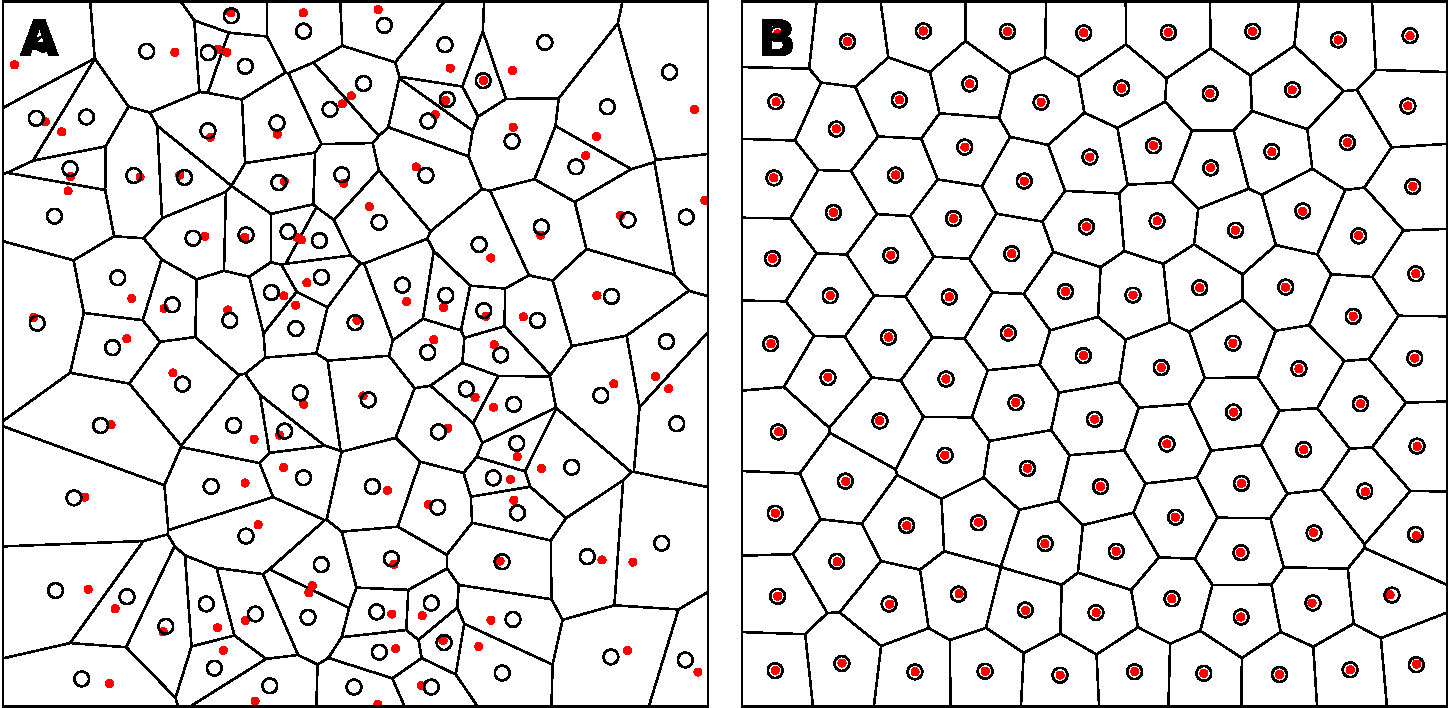
\includegraphics[width=\textwidth]{figures/CVT.pdf}
%%   \caption{\textbf{Centroidal Voronoi Tesselation.}  \textbf{\textsf{A.}}
%%     Voronoi diagram of a uniform distribution (n=100) where red dots represent
%%     the uniform distribution and white circles represent the centroids of each
%%     Voronoi cell. \textbf{\textsf{B.}} Centroidal Voronoi diagram where the
%%     point distribution matches the centroid distribution which constitutes a
%%     blue noise distribution (i.e. {\em a distribution that is roughly uniformly
%%       random with no preferred inter-point directions or distances} according
%%     to the definition of \cite{Ebeida:2014}). This figure has been obtained
%%     from the initial distribution on the left after 50 iterations of the Lloyd
%%     relaxation algorithm. }
%%   \label{fig:CVT}
%% \end{figure}
%
